\documentclass[a4paper]{article}
\usepackage[left=2cm,right=2cm,top=3cm,bottom=3cm]{geometry}
\usepackage[T1]{fontenc}
\usepackage{amsmath}
\usepackage{mathtools}
\usepackage{amssymb}
\usepackage{indentfirst}
\usepackage{graphicx}
\usepackage{amsthm}
\usepackage{interval}
\usepackage{algorithm}
\usepackage{algorithmic}
\usepackage{subfigure}

\graphicspath{ {./images/} }
\newtheorem{theorem}{Theorem}

\title{\textbf{Pracownia z Analizy Numerycznej}\\{\Large Sprawozdanie do zadania P2.10}}
\author{Mateusz Leonowicz}

\newcommand{\RomanNumeralCaps}[1]
    {\MakeUppercase{\romannumeral #1}}

\begin{document}
\maketitle
\section{Wstęp}
    Częstym problemem, który pojawia się podczas pracy przy różnego rodzaju funkcjach
    jest trudność w ich różniczkowaniu i całkowaniu. Musimy mieć możliwość wykonywania tych operacji bez wstępnej analizy funkcji,
    czy też jej przekształcenia. Chcemy więc zamienić naszą skomplikowaną funkcję na jakąś inną (najlepiej wielomianową), która dobrze
    ją przybliża. Jest to jedno z podstawowych zagadnień analizy numerycznej. 

    W naszym zadaniu spojrzymy na problem z całkowaniem funkcji. 
    W ogólności dla dowolnej funkcji $f$, dwóch wartości $a \leq b$ chcemy policzyć wartość funkcji $\phi$:
    \[
        \Phi (x) = \int_{a}^{x} f(t) \, dt \quad \text{dla} \quad a \leq x \leq b.
    \]
    korzystając z interpolujących naturalnych funkcji sklejanych \RomanNumeralCaps{3} stopnia.

\tableofcontents

\newpage
\section{Naturalna funkcja sklejana \RomanNumeralCaps{3} stopnia.}
    Niech dana będzie interpolowana funkcja $f$ ciągła na przedziale $\interval[]{a}{b}$ oraz $n+1$ węzłów 
    $t_0, t_1, \dotsc, t_n$ \newline takich, że $a = t_0 < t_1 < t_2 < \dotsc < t_n = b$. Naturalną funkcją sklejaną 
    \RomanNumeralCaps{3} stopnia będzie taka funkcja $S$, dla której spełnione są warunki:
    \begin{itemize}
        \item W każdym z przedziałów $\interval[]{t_i}{t_{i+1}} \ (0 \leq i \leq n - 1)$ S jest wielomianem klasy $\Pi_3$.
        \item Funkcje $S$, $S'$ i $S''$ są ciągłe w przedziale $\interval[]{a}{b}$.
        \item $S(t_i) = f(t_i) \ (0 \leq i \leq n)$
        \item $S''(a) = S''(b) = 0$ (Warunek na $S$ naturalne)
    \end{itemize}

    Jeśli chcemy mieć jednoznacznie wyznaczoną funkcję, to z pierwszego punktu wynika, że potrzebujemy dokładnie $4n$ warunków
    na istnienie $S$. Sprawdźmy czy tak jest. Z drugiego punktu, który zapewnia, że zachodzą równości:
    \begin{equation}     
        \label{1}   
        \begin{aligned}  
            S'_{i-1}(t_i) &= S'_i(t_i) \quad (1 \leq i \leq n-1) \\
            S''_{i-1}(t_i) &= S''_i(t_i) \quad (1 \leq i \leq n-1)
        \end{aligned}
    \end{equation}
    otrzymujemy dokładnie $2(n-1)$ warunków dla naszej funkcji S. Z trzeciego punktu mamy $2n$ warunków,
    a z ostatniego $2$. Mamy więc wystarczającą ilość informacji, aby wprost stworzyć naszą funkcję.
    
    Znajdźmy napierw wzór na $S_i(x)$ w przedziale $\interval[]{t_i}{t_{i+1}}$. Wprowadzamy nowe oznaczenie $\lambda_i = S''(t_i)$.
    \newline Wiemy, że $S_i \in \Pi_3$ więc funkcja $S''_i$ jest funkcją liniową. Z równości $S''_i(t_i) = \lambda_i$ i $S''_i(t_{i+1}) = \lambda_{i+1}$ wynika, że:
    \[
          S''_i(x) = \frac{\lambda_i}{t_{i+1} - t_i}(t_{i+1} - x) + \frac{\lambda_{i+1}}{t_i - t_{i+1}}(t_i - x)
    \]
    Jest to oczywiście wielomian interpolacyjny dla węzłów $t_i, t_{i+1}$ w postaci Lagrange'a. Dla ułatwienia przekształceń niech $h_i = t_{i+1} - t_i$. 
    Jeśli zcałkujemy obie strony dwukrotnie otrzymamy wielomian $S_i$.
    \[
        \begin{split}
            \int S''_i(x) \, dx  & = \int \frac{\lambda_i}{h_i}(t_{i+1} - x) \, dx + \int \frac{\lambda_{i+1}}{h_i}(x - t_i) \, dx \\
                                 & = \frac{-\lambda_i}{2h_i}(t_{i+1} - x)^2 + \frac{\lambda_{i+1}}{2h_i}(x - t_i)^2 + C \\
                                 & = S'_i(x)
        \end{split}
    \]
    \[
        \begin{split}
            \int \int S''_i(x) \, dx \, dx & = \int \frac{-\lambda_i}{2h_i}(t_{i+1} - x)^2 \, dx + \int \frac{\lambda_{i+1}}{2h_i}(x - t_i)^2 + C \, dx \\
                                           & = \frac{\lambda_i}{6h_i}(t_{i+1} - x)^3 + \frac{\lambda_{i+1}}{6h_i}(x - t_i)^3 + Cx + D \\
                                           & = S_i(x)
        \end{split}  
    \]
    Teraz pozostaje wyznaczyć stałe całkowania $C$ i $D$ z równości $S_i(t_i) = f(t_i)$ oraz $S_i(t_{i+1}) = f(t_{i+1})$.
    \[
        \begin{aligned}
            & S_i(t_i) = \frac{\lambda_i}{6h_i}(t_{i+1} - t_i)^3 + t_iC + D = f(t_i) \\
            & S_i(t_{i+1}) = \frac{\lambda_{i+1}}{6h_i}(t_{i+1} - t_i)^3 + t_{i+1}C + D = f(t_{i+1})
        \end{aligned}
    \]
    Rozwiązując ten układ równań otrzymujemy postać naszej funkcji sklejanej.
    \begin{equation}
        \label{2}
        S_i(x) = \frac{\lambda_i}{6h_i}(t_{i+1} - x)^3 + \frac{\lambda_{i+1}}{6h_i}(x - t_i)^3 + 
        \bigg(\frac{f(t_{i+1})}{h_i} - \frac{\lambda_{i+1}h_i}{6}\bigg)(x - t_i) +
        \bigg(\frac{f(t_{i})}{h_i} - \frac{\lambda_ih_i}{6}\bigg)(t_{i+1} - x)
    \end{equation}
    Musimy jeszcze wyznaczyć wartości $\lambda_1, \lambda_2, \dotsc, \lambda_{n-1}$ tak, aby zapewnić ciągłość pierwszej pochodnej.
    Aby to zrobić zróżniczkujemy wielomian \eqref{2} i skorzystamy z równości \eqref{1}.

\newpage
    Otrzymujemy:
    \[
        \begin{aligned}
            & S'_i(x) = \frac{-\lambda_i}{2h_i}(t_{i+1} - x)^2 + \frac{\lambda_{i+1}}{2h_i}(x - t_i)^2
            + \bigg(\frac{f(t_{i+1})}{h_i} - \frac{\lambda_{i+1}h_i}{6}\bigg)
            - \bigg(\frac{f(t_{i})}{h_i} - \frac{\lambda_ih_i}{6}\bigg) \\
            & S'_{i-1}(x) = \frac{-\lambda_{i-1}}{2h_{i-1}}(t_{i} - x)^2 + \frac{\lambda_{i}}{2h_{i-1}}(x - t_{i-1})^2
            + \bigg(\frac{f(t_{i})}{h_{i-1}} - \frac{\lambda_{i}h_{i-1}}{6}\bigg)
            - \bigg(\frac{f(t_{i-1})}{h_{i-1}} - \frac{\lambda_{i-1}h_{i-1}}{6}\bigg) 
        \end{aligned}
    \]
    i podstawiajac $x = t_i$ dostajemy:
    \[
        \begin{aligned}
            & S'_i(t_i) = -\frac{h_i}{3}\lambda_i - \frac{h_i}{6}\lambda_{i+1} - \frac{f(t_i)}{h_i} + \frac{f(t_{i+1})}{h_i} \\
            & S'_{i-1}(t_i) = \frac{h_{i-1}}{6}\lambda_{i-1} + \frac{h_{i-1}}{3}\lambda_{i} - \frac{f(t_{i-1})}{h_{i-1}} + \frac{f(t_{i})}{h_{i-1}}
        \end{aligned}
    \]
    Przyrównujemy do siebie dwa wyrażenia:
    \[
        h_{i-1}\lambda_{i-1} + 2(h_{i-1} + h_i)\lambda_i + h_i\lambda_{i+1} = \frac{6}{h_i}(f(t_{i+1}) - f(t_i)) - \frac{6}{h_{i-1}}(f(t_i) - f(t_{i-1}))
    \]
    Dostaliśmy więc układ $n-1$ równań dla $n-1$ niewiadomych $\lambda_1, \lambda_2, \dotsc, \lambda_{n-1}$. Możemy rozwiązać ten układ, \newline a otrzymane
    wyniki wykorzystać do konstrukcji naszego wielomianu.

    Wprowadzamy nowe oznaczenia:
    \[
        u_i = 2(h_{i-1} + h_i), \quad b_i = \frac{6}{h_i}(f(t_{i+1}) - f(t_i)), \quad v_i = b_i - b_{i-1}
    \]
    Pamiętając, że $\lambda_0 = \lambda_n = 0$ nasz układ przedstawia się w postaci macierzowej:
    \[
        \begin{bmatrix}
            u_1 & h_1 & & & \\
            h_1 & u_2 & h_2 & & \\
                & \ddots & \ddots & \ddots & \\
                & & h_{n-3} & u_{n-2} & h_{n-2} \\
                & & & h_{n-2} & u_{n-1}
        \end{bmatrix}
        \begin{bmatrix}
            \lambda_1 \\
            \lambda_2 \\
            \vdots \\
            \lambda_{n-2} \\
            \lambda_{n-1}
        \end{bmatrix}
        =
        \begin{bmatrix}
            v_1 \\
            v_2 \\
            \vdots \\
            v_{n-2} \\
            v_{n-1}
        \end{bmatrix}
    \]
    Teraz stosując eliminację Gaussa możemy w prosty sposób rozwiązać ten układ równań. Algorytm możemy wyrazić w sposób następujący.
    \vspace{5mm}
    \begin{algorithm}
        \caption{Wyznaczanie wartości $\lambda_i$}
        \begin{algorithmic}
        \REQUIRE $n, (t_i), f(t_i)$
            \FOR{$i = 0:n - 1$}
                \STATE $h_i \leftarrow t_{i+1} - t_i$
                \STATE $b_i \leftarrow \frac{6(f(t_{i+1}) - f(t_i))}{h_i}$
            \ENDFOR
            \STATE $u_1 \leftarrow 2(h_0 + h_1)$
            \STATE $v_1 \leftarrow b_1 - b_0$
            \FOR{$i = 2:n - 1$}
                \STATE $u_i \leftarrow 2(h_{i-1} + h_i) - \frac{h_{i-1}^2}{u_{i-1}}$
                \STATE $v_i \leftarrow b_i - b_{i-1} - \frac{h_{i-1}v_{i-1}}{u_{i-1}}$
            \ENDFOR
            \STATE $\lambda_0 \leftarrow 0$
            \STATE $\lambda_n \leftarrow 0$
            \FOR{$i = n - 1:1$}
                \STATE $\lambda_i \leftarrow \frac{(v_i - h_i\lambda_{i+1})}{u_i}$
            \ENDFOR
            \STATE $\text{return} \ \ \lambda$
        \end{algorithmic}
    \end{algorithm}

\newpage
\section{Całkowanie funkcji sklejanej \RomanNumeralCaps{3} stopnia.}
    W drugiej części zadania chcemy obliczyć wartość całki $\Phi'(x)$ danej wzorem:
    \[
        \Phi'(x) = \int_{a}^{x} S(t) \approx \Phi(x)\, dt  
    \]
    wiedząc, że $S(t)$ jest naturalną funkcją sklejaną \RomanNumeralCaps{3} stopnia, oraz znając najmniejsze takie $t_k$, że $x \leq t_k$
    możemy naszą całkę podzielić na sumę całek w następujący sposób:
    \[
        \Phi'(x) = \int_{t_0}^{t_1} S_0(u) \, du + \int_{t_1}^{t_2} S_1(u) \, du + \dotsc + \int_{t_k}^{x} S_k(u) \, du
    \]

    Następnie, aby ułatwić nam wyznaczenie $S_i$ przekształcimy wzór \eqref{2} na taki, który pozwoli nam w łatwy sposób policzyć
    współczynniki wielomianu.
    \[
        \begin{split}
            S_i(x) & = \frac{\lambda_i}{6h_i}(t_{i+1} - x)^3 + \frac{\lambda_{i+1}}{6h_i}(x - t_i)^3 + 
                \bigg(\frac{f(t_{i+1})}{h_i} - \frac{\lambda_{i+1}h_i}{6}\bigg)(x - t_i) +
                \bigg(\frac{f(t_{i})}{h_i} - \frac{\lambda_ih_i}{6}\bigg)(t_{i+1} - x) \\
                  & = x^3\bigg(-\frac{\lambda_i}{6h} + \frac{\lambda_{i+1}}{6h}\bigg) +
                  x^2\bigg(\frac{\lambda_i}{2h}t_{i+1} - \frac{\lambda_{i+1}}{2h}t_i\bigg) + \\
                  & + x\bigg(-\frac{-\lambda_i}{2h}t_{i+1}^2 + \frac{\lambda_{i+1}}{2h}t_i^2 + \frac{f(t_{i+1})}{h} -
                  \frac{\lambda_{i+1}h}{6} - \frac{f(t_i)}{h} + \frac{\lambda_ih}{6}\bigg) \\
                  & + \frac{\lambda_i}{6h}t_{i+1}^3 - \frac{\lambda_{i+1}}{6h}t_i^3 - \frac{f(t_{i+1})}{h}t_i
                  + \frac{\lambda_{i+1}h}{6}t_i + \frac{f(t_i)}{h}t_{i+1} - \frac{\lambda_ih}{6}t_{i+1}
        \end{split}
    \]
    Reszta obliczeń polega na wykorzystaniu powyższych własności i podstawieniu odpowiednich wartości.

\section{Testy numeryczne}
    W tej sekcji sprawdzać będziemy jak skuteczną metodą przybliżania wartości całki jest całkowanie funkcji sklejanej \RomanNumeralCaps{3} stopnia.
    Policzę przybliżenia wartości całek oraz ich błąd bezwzględny uwzględniając różne ilości przedziałów. Dodatkowo pokażę ile potrzebujemy przedziałów,
    aby uzyskać satysfakcjonujący błąd (jeśli to możliwe).

\newpage
\subsection{Test 1}
    Funkcja przykładowa, aby zaprezentować sposób prezentacji danych oraz kryteria porównawcze.
    \[
        \begin{aligned}
            x &= 2.4 \\
            a &= 0 \\
            b &= 4 \\
            f(x) &= 5sin(x) + \frac{1}{10}x^2 + 50cos(x) + log(x + 5) \\
            \Phi(x) &= 47.284690044648194
        \end{aligned}
    \]

    \begin{center}
        \begin{tabular}{|c|c|c|} 
            \hline
            n & $\Phi'(x)$ & Błąd bezwzględny \\
            \hline
            2 & -20.582009632895932 & 67.86669967754412 \\
            \hline
            3 & 34.00320421138793 & 13.281485833260263 \\
            \hline
            5 & 46.63022254583059 & 0.6544674988176027 \\
            \hline
            20 & 47.205650943683715 & 0.0790391009644793\\
            \hline
            100 & 46.01890472357011 & 1.2657853210780843 \\
            \hline
            130 & 47.28465506244014 & 3.498220805653318e-5 \\
            \hline
        \end{tabular}
    \end{center}

    \begin{figure}[!htbp]
        \hfill
        \subfigure[$n = 2$]{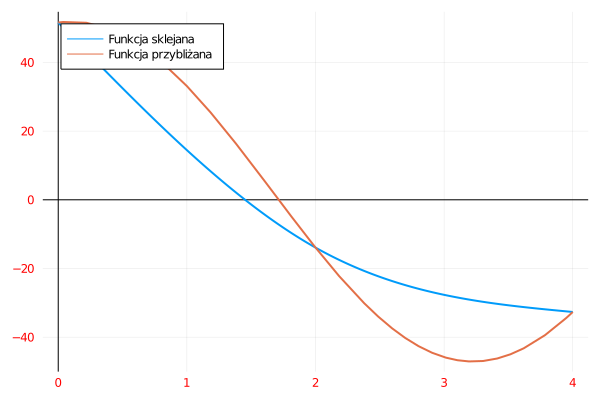
\includegraphics[width=8cm]{12}}
        \hfill
        \subfigure[$n = 3$]{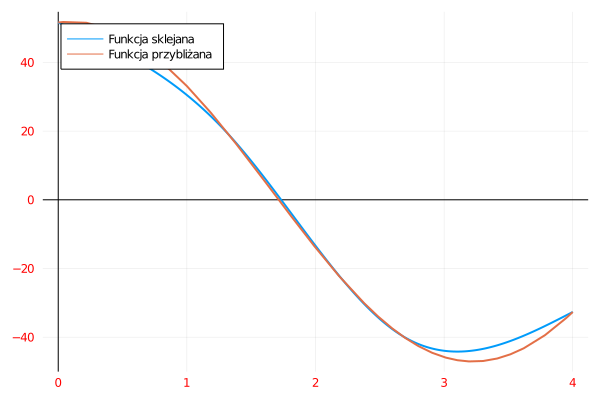
\includegraphics[width=8cm]{13}}
        \hfill
    \end{figure}
    \begin{figure}[!htbp]
        \hfill
        \subfigure[$n = 5$]{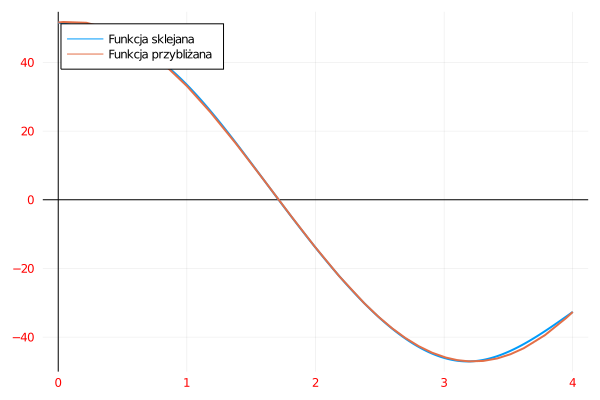
\includegraphics[width=8cm]{15}}
        \hfill
        \subfigure[$n = 20$]{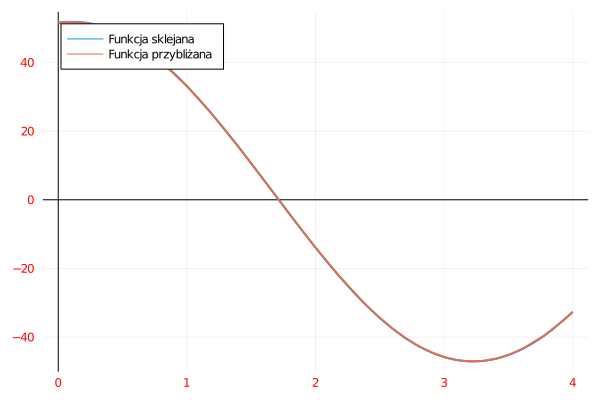
\includegraphics[width=8cm]{120}}
        \hfill
    \end{figure}
    
    Widzimy, że aby otrzymać 2 cyfry znaczące potrzebowaliśmy złożyć ze sobą 20 wielomianów. Co ciekawe, dla coraz
    większej liczby przedziałów wartość naszej całki zaczęła coraz bardziej różnić się od wartości przybliżanej. Dopiero w okolicy 
    100 funkcji sklejanych otrzymaliśmy błąd rzędu 5 cyfr znaczących.

\newpage
\subsection{Test 2}
    Funkcja która wygląda na okresową, ale z przesuniętym każdym okresem w górę.
    \[
        \begin{aligned}
            x &= 3 \\
            a & = 0 \\
            b &= 5 \\
            f(x) &= sin(5x) + \exp(\frac{x}{5}) - 3 \\
            \Phi(x) &= -4.537468415475691
        \end{aligned}
    \]

    \begin{center}
        \begin{tabular}{|c|c|c|} 
            \hline
            n & $\Phi'(x)$ & Błąd bezwzględny \\
            \hline
            2 & -6.693193 & 2.155724 \\
            \hline
            5 & -6.331958 & 1.794490 \\
            \hline
            10 & -5.317852 & 0.780384 \\
            \hline
            20 & -4.803045 & 0.265577 \\
            \hline
            50 & -4.609706 & 0.072237 \\
            \hline
            250 & -4.548728 & 0.011260 \\
            \hline
            1000 & -4.540150 & 0.002681 \\
            \hline
            50000 & -4.537521 & 0.000053 \\
            \hline
        \end{tabular}
    \end{center}

    \begin{figure}[!htbp]
        \hfill
        \subfigure[$n = 2$]{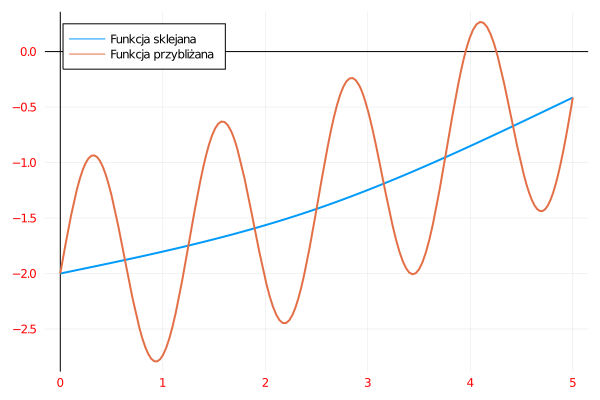
\includegraphics[width=8cm]{22}}
        \hfill
        \subfigure[$n = 5$]{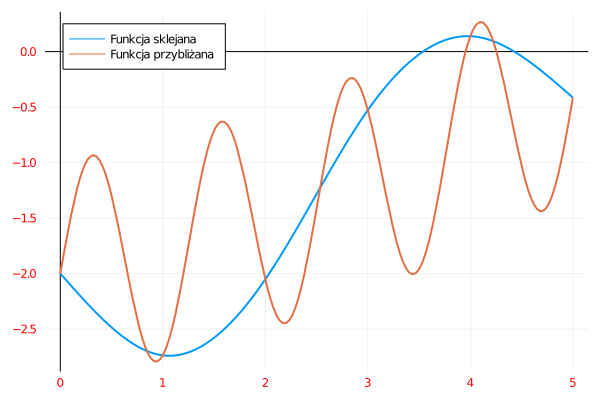
\includegraphics[width=8cm]{25}}
        \hfill
    \end{figure}
    \begin{figure}[!htbp]
        \hfill
        \subfigure[$n = 10$]{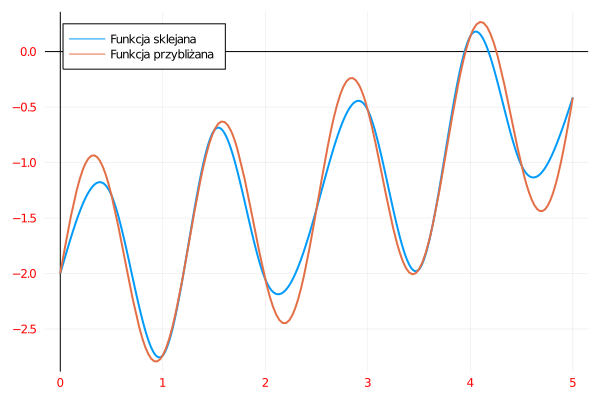
\includegraphics[width=8cm]{210}}
        \hfill
        \subfigure[$n = 20$]{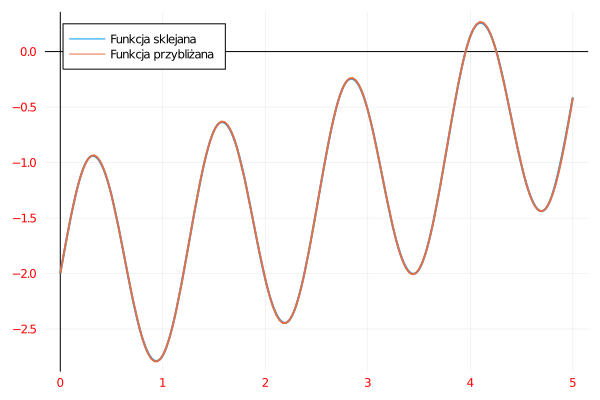
\includegraphics[width=8cm]{220}}
        \hfill
    \end{figure}
    
    Do otrzymania jednej cyfry znaczącej potrzebowaliśmy jedynie 10 wielomianów, ale aby uzyskać każdą kolejną cyfrę
    potrzebowaliśmy wykonywać coraz to więcej operacji. Do uzyskania 5 cyfr znaczących potrzebowaliśmy już 50000 wielomianów
    co może sugerować, że zbieżnośc tej metody potrafi być naprawdę słaba.

\newpage
\subsection{Test 3}
    Funkcja Rungego, która znana jest z tego, że sprawia problem w klasycznej interpolacji.
    \[
        \begin{aligned}
            x &= 1.5 \\
            a & = -2 \\
            b &= 2 \\
            f(x) &= \frac{1}{1 + 25x^2} \\
            \Phi(x) &= 0.5818744937603915
        \end{aligned}
    \]

    \begin{center}
        \begin{tabular}{|c|c|c|} 
            \hline
            n & $\Phi'(x)$ & Błąd bezwzględny \\
            \hline
            2 & 2.514851 & 1.932977 \\
            \hline
            5 & 0.366765 & 0.215109 \\
            \hline
            10 & 0.640139 & 0.058265 \\
            \hline
            15 & 0.574224 & 0.007651 \\
            \hline
            20 & 0.585868 & 0.003993 \\
            \hline
            40 & 0.583519 & 0.001644 \\
            \hline
            100 & 0.582219 & 0.000345 \\
            \hline
            1000 & 0.581944 & 0.000070 \\
            \hline
        \end{tabular}
    \end{center}

    \begin{figure}[!htbp]
        \hfill
        \subfigure[$n = 2$]{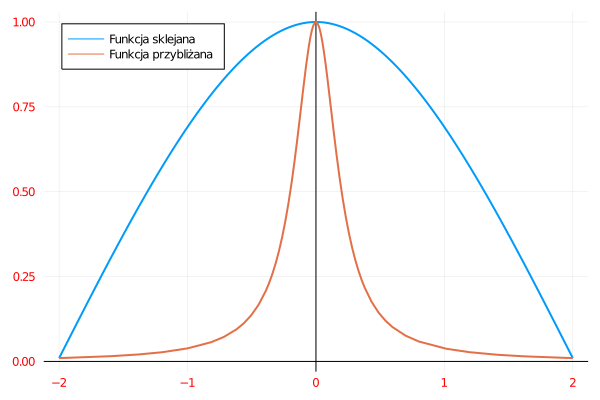
\includegraphics[width=8cm]{32}}
        \hfill
        \subfigure[$n = 5$]{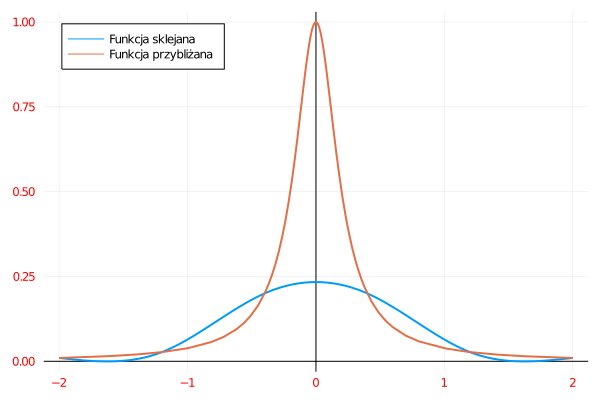
\includegraphics[width=8cm]{35}}
        \hfill
    \end{figure}
    \begin{figure}[!htbp]
        \hfill
        \subfigure[$n = 10$]{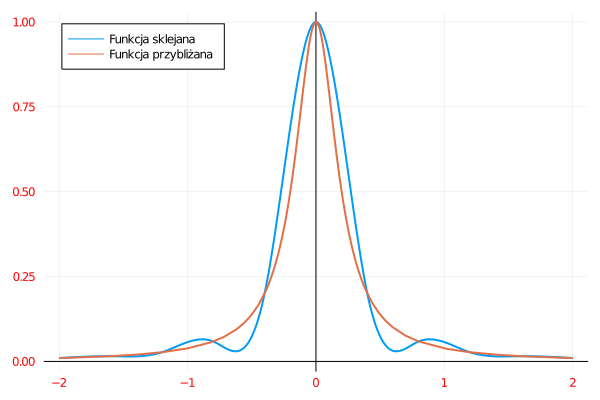
\includegraphics[width=8cm]{310}}
        \hfill
        \subfigure[$n = 15$]{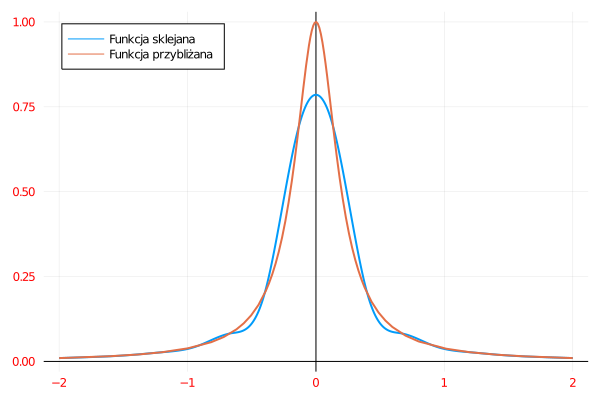
\includegraphics[width=8cm]{315}}
        \hfill
    \end{figure}
    
    Widzimy, że metoda funkcji sklejanej dobrze radzi sobie z funkcją Rungego i już dla 10 wielomianów otrzymaliśmy 2 cyfry znaczące.
    Problemem jednak niestety znów jest rząd zbieżności, aby otrzymać chociaż 5 cyfr znaczących musieliśmy użyć aż 1000 wielomianów.

\newpage
\subsection{Test 4}
    Zwykły wielomian 5 stopnia.
    \[
        \begin{aligned}
            x &= 1.3 \\
            a & = 0 \\
            b &= 2 \\
            f(x) &= \frac{x^5}{1000} - \frac{x^3}{32} + \frac{2x}{13} \\
            \Phi(x) &= 0.10849118691666668
        \end{aligned}
    \]

    \begin{center}
        \begin{tabular}{|c|c|c|} 
            \hline
            n & $\Phi'(x)$ & Błąd bezwzględny \\
            \hline
            2 & 0.188130 & 0.079639 \\
            \hline
            3 & 0.113336 & 0.004845 \\
            \hline
            5 & 0.148603 & 0.040112 \\
            \hline
            10 & 0.122012 & 0.013521 \\
            \hline
            50 & 0.111194 & 0.002703 \\
            \hline
            100 & 0.111194 & 0.002703 \\
            \hline
            1000 & 0.108761 & 0.000270 \\
            \hline
            10000 & 0.108518 & 0.000027 \\
            \hline
        \end{tabular}
    \end{center}

    \begin{figure}[!htbp]
        \hfill
        \subfigure[$n = 2$]{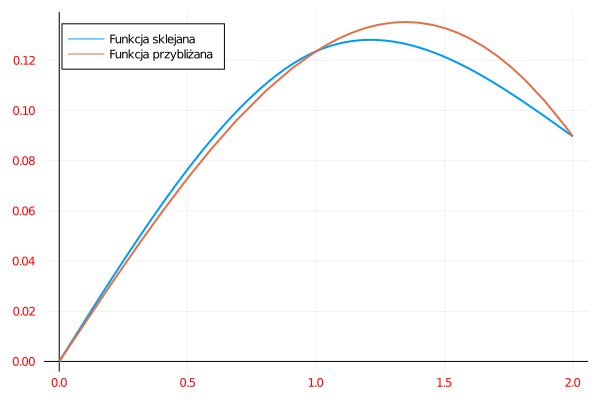
\includegraphics[width=8cm]{42}}
        \hfill
        \subfigure[$n = 5$]{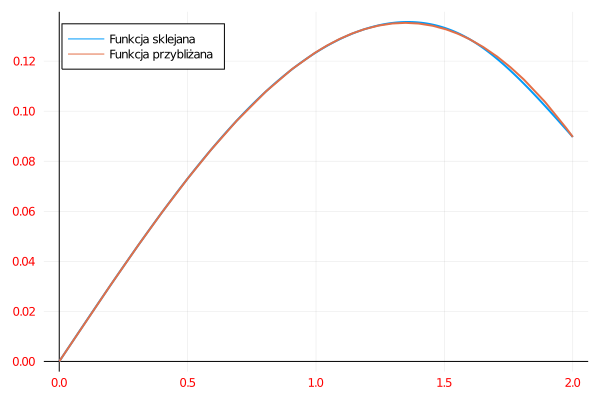
\includegraphics[width=8cm]{45}}
        \hfill
    \end{figure}
    
   Funkcja sklejana dobrze przybliża wielomian już w niewielkiej liczbie sklejonych wielomianów. Pomimo tego, że już przy 2 wielomianach
   dostaliśmy 2 cyfry znaczące, to żeby dostać ich 5 potrzebowaliśmy aż 10000 wielomianów. Zaskakujące jest, że nasza metoda tak słabo wypada
   nawet dla wielomianów podobnego stopnia co funkcja sklejana. Nie jest to dobra własność, jeżeli chcemy móc liczyć wartości całek z każdej funkcji.  

\newpage
\subsection{Test 5}
    Funkcja, której granica w zerze wynosi minus nieskończoność.
    \[
        \begin{aligned}
            x &= 1.7 \\
            a & = 0.05 \\
            b &= 2 \\
            f(x) &= -(sin(x) + \frac{1}{250x^2}) \\
            \Phi(x) &= -1.2052418135140226
        \end{aligned}
    \]

    \begin{center}
        \begin{tabular}{|c|c|c|} 
            \hline
            n & $\Phi'(x)$ & Błąd bezwzględny \\
            \hline
            2 & -1.982424 & 0.777182 \\
            \hline
            5 & -1.672953 & 0.467711 \\
            \hline
            10 & -1.377668 & 0.172426 \\
            \hline
            20 & -1.234317 & 0.029076 \\
            \hline
            50 & -1.235133 & 0.029891 \\
            \hline
            150 & -1.235133 & 0.029891 \\
            \hline
            1000 & -1.206881 & 0.001639 \\
            \hline
            10000 & -1.205331 & 0.000089 \\
            \hline
        \end{tabular}
    \end{center}

    \begin{figure}[!htbp]
        \hfill
        \subfigure[$n = 2$]{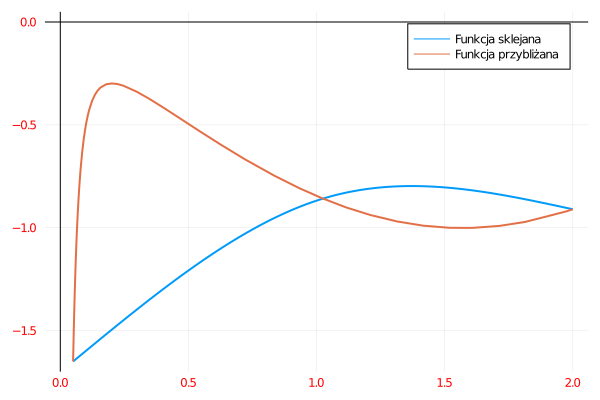
\includegraphics[width=8cm]{52}}
        \hfill
        \subfigure[$n = 5$]{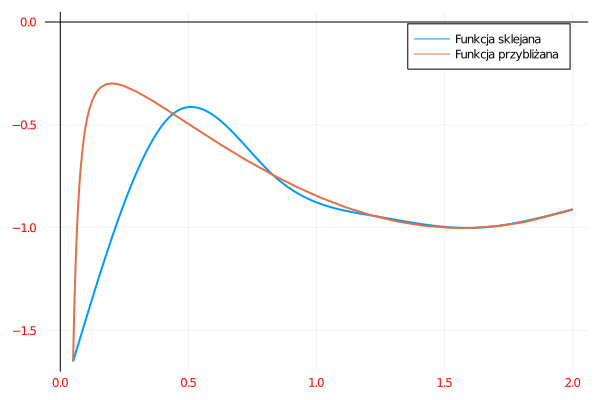
\includegraphics[width=8cm]{55}}
        \hfill
    \end{figure}
    \begin{figure}[!htbp]
        \hfill
        \subfigure[$n = 10$]{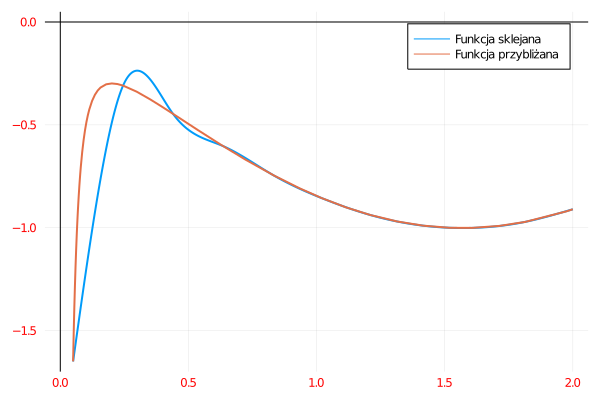
\includegraphics[width=8cm]{510}}
        \hfill
        \subfigure[$n = 20$]{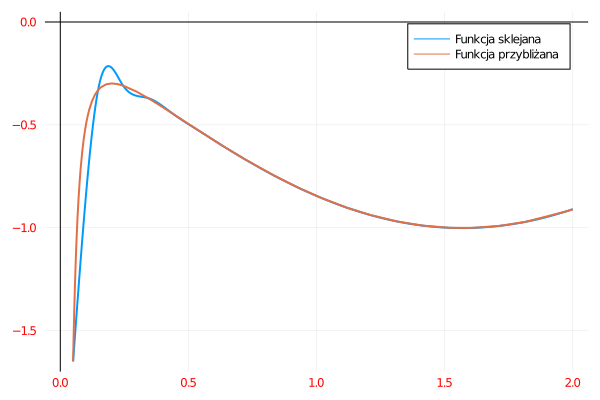
\includegraphics[width=8cm]{520}}
        \hfill
    \end{figure}
    
   Znów, nawet dla niezbyt skomplikowanej funkcji szybko otrzymaliśmy 2 cyfry znaczące, ale żeby otrzymać dokładność do 5 cyfr znaczących
   musieliśmy wyznaczyć aż 10000 wielomianów.

\newpage
\subsection{Test 6}
    Funkcja bardzo szybko zmieniająca swoje wartości w krótkim przedziale.
    \[
        \begin{aligned}
            x &= 0.9 \\
            a & = 0.25 \\
            b &= 1 \\
            f(x) &= sin(\frac{1}{1 + x^2}) \\
            \Phi(x) &= 0.11994153632149726
        \end{aligned}
    \]

    \begin{center}
        \begin{tabular}{|c|c|c|} 
            \hline
            n & $\Phi'(x)$ & Błąd bezwzględny \\
            \hline
            2 & 0.090881 & 0.029060 \\
            \hline
            5 & 0.253998 & 0.134057 \\
            \hline
            15 & 0.124974 & 0.005032 \\
            \hline
            30 & 0.144286 & 0.024344 \\
            \hline
            50 & 0.130445 & 0.010504 \\
            \hline
            100 & 0.122524 & 0.002582 \\
            \hline
            1000 & 0.120190 & 0.000248 \\
            \hline
            10000 & 0.119966 & 0.000025 \\
            \hline
        \end{tabular}
    \end{center}

    \begin{figure}[!htbp]
        \hfill
        \subfigure[$n = 2$]{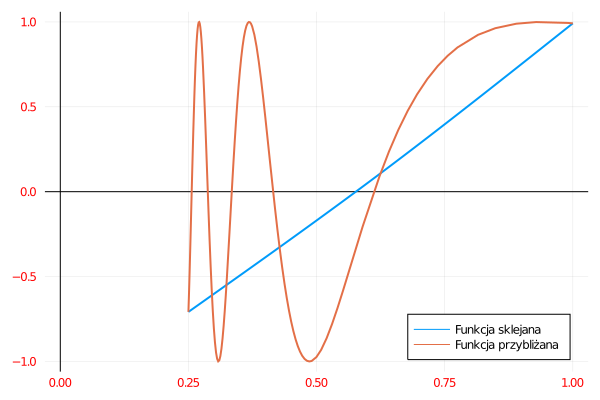
\includegraphics[width=8cm]{62}}
        \hfill
        \subfigure[$n = 5$]{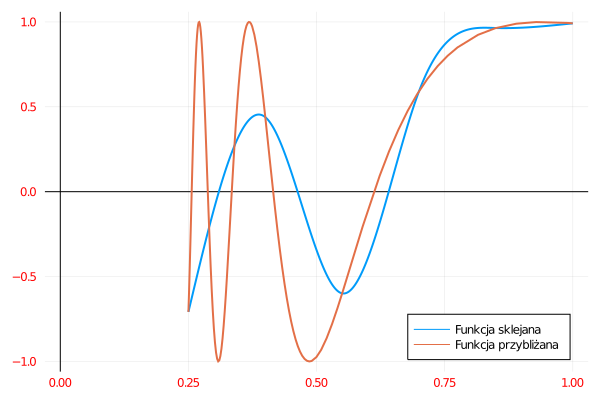
\includegraphics[width=8cm]{65}}
        \hfill
    \end{figure}
    \begin{figure}[!htbp]
        \hfill
        \subfigure[$n = 15$]{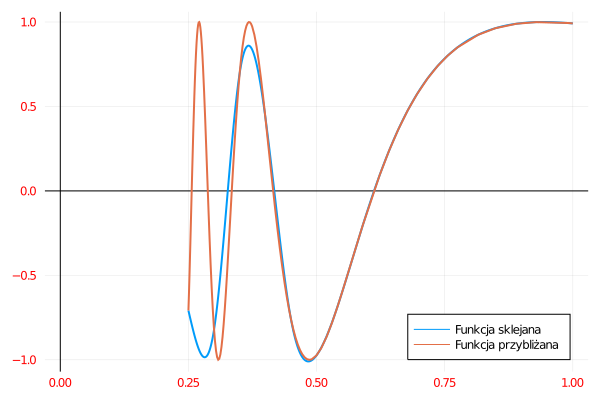
\includegraphics[width=8cm]{615}}
        \hfill
        \subfigure[$n = 30$]{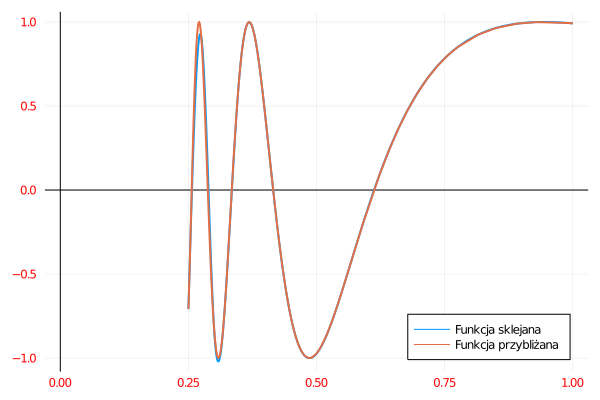
\includegraphics[width=8cm]{630}}
        \hfill
    \end{figure}
    
   Ponownie otrzymaliśmy bardzo szybko 2 cyfry znaczące, ale żeby uzyskać ich więcej musimy wykonać bardzo dużo obliczeń.
   Jeszcze raz 10000 wielomianów okazało się wystarczające, żeby obliczyć 5 cyfrę znaczącą. Możnaby podejrzewać, że jest to
   własność tej metody.

\newpage
\subsection{Test 7}
    Funkcja nie będąca różniczkowalna w każdym punkcie swojej dziedziny.
    \[
        \begin{aligned}
            x &= 0 \\
            a & = -\pi \\
            b &= \pi \\
            f(x) &= |sin(x)| - exp(\frac{1}{x^{100}}) \\
            \Phi(x) &= 1.0056741488084917
        \end{aligned}
    \]

    \begin{center}
        \begin{tabular}{|c|c|c|} 
            \hline
            n & $\Phi'(x)$ & Błąd bezwzględny \\
            \hline
            2 & -3.926991 & 4.932665 \\
            \hline
            10 & 0.515500 & 0.490174 \\
            \hline
            25 & 0.884451 & 0.121223 \\
            \hline
            100 & 1.014446 & 0.008772 \\
            \hline
            200 & 1.006806 & 0.001132 \\
            \hline
            400 & 1.005646 & 0.000028 \\
            \hline
            10000 & 1.005046 & 0.000628 \\
            \hline
        \end{tabular}
    \end{center}

    \begin{figure}[!htbp]
        \hfill
        \subfigure[$n = 2$]{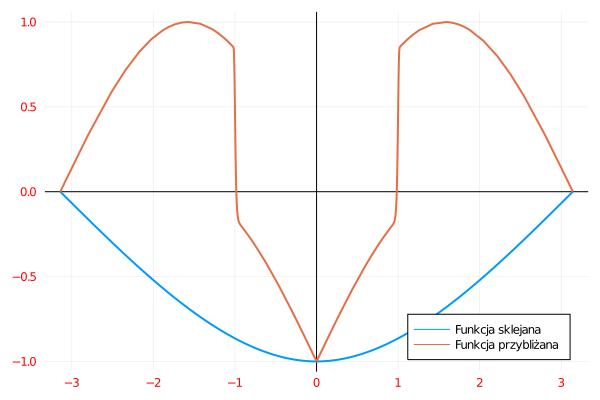
\includegraphics[width=8cm]{72}}
        \hfill
        \subfigure[$n = 10$]{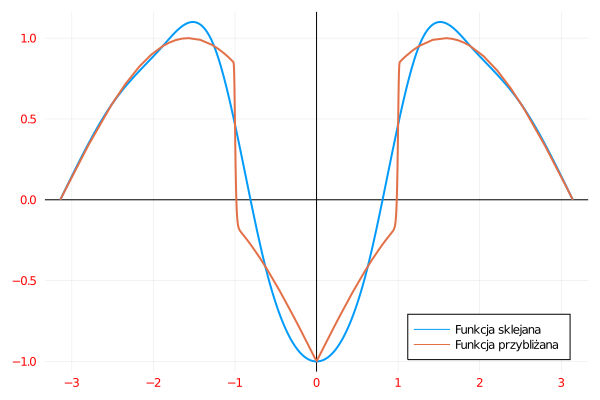
\includegraphics[width=8cm]{710}}
        \hfill
    \end{figure}
    \begin{figure}[!htbp]
        \hfill
        \subfigure[$n = 25$]{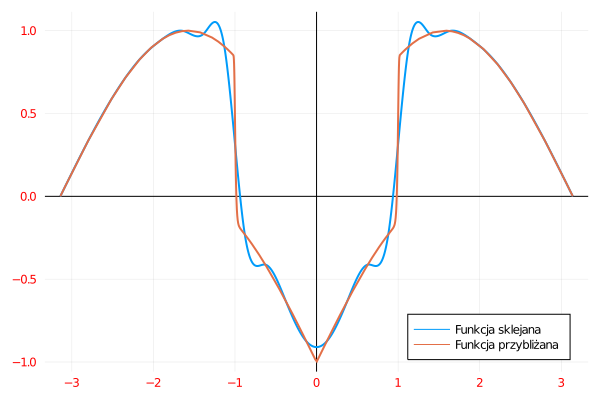
\includegraphics[width=8cm]{725}}
        \hfill
        \subfigure[$n = 100$]{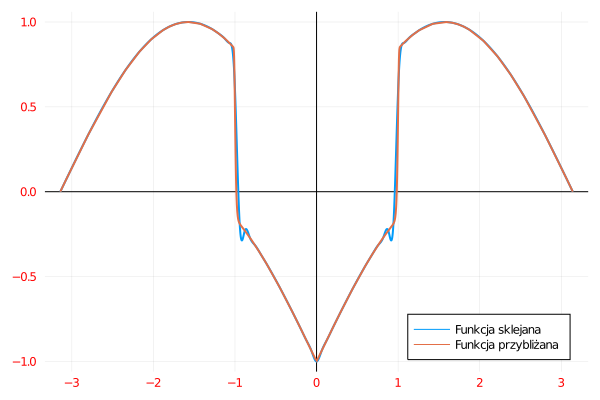
\includegraphics[width=8cm]{7100}}
        \hfill
    \end{figure}
    
   Metoda bardzo dobrze poradziła sobie z odtworzeniem własności funkcji oraz z przybliżeniem jej w danym przedziale.
   Niestety zbieżnośc wartości całki znów pozostawia wiele do życzenia. Pożądaną zbieżnośc 5 cyfr znaczących otrzymaliśmy
   dopiero przy użyciu 400 wielomianów. Co ciekawe zwiększenie tej liczby do 10000 zwiększyło nasz błąd bezwzględny. Może być to spowodowane
   błędnami numerycznymi.

\newpage
\section{Podsumowanie}
    Wykonane przeze mnie testy pokazują skuteczność metody przybliżania wartości całki za pomocą funkcji sklejanych 
    \RomanNumeralCaps{3} stopnia. Funkcje te bardzo dobrze i szybko zbiegają do funkcji interpolowanej. Możemy dzięki nim 
    poznać kształt oraz ogólne własności funkcji o której chcemy się czegoś dowiedzieć. Niestety, jeśli przychodzi nam wyliczać 
    za jej pomocą wartość całki to metoda ta nie sprawdza się. Pomimo tego że pierwsze cyfry znaczące otrzymujemy prawie natychmiastowo
    to uzyskanie każdej kolejnej cyfry znaczącej wymaga dużego nakładu obliczeniowego, co oznacza, że metoda nie jest efektywnym
    sposobem wyznaczania wartości całek jeśli zależy nam na dużej dokładności. Jeśli jednak chcemy uzyskać jedynie rząd, albo
    pozwalamy na to, aby błąd bezwzględny był zauważalnie duży, to metoda ta może nam bardzo dobrze służyć.

    Podsumowując więc, metoda ta stanowi raczej ciekawostkę, aniżeli pełnoprawną i użyteczną metodę wyznaczania wartości całki w przedziale.

    \begin{thebibliography}{9}
        \bibitem{Kincaid}
        David Kincaid, Ward Cheney. 
        Analiza numeryczna, Warszawa, 2006..
    \end{thebibliography} 
\end{document}
